%%%%%%%%%%%%%%%%%%%%%%%%%%%%%%%%%
% Results and Findings          %
%%%%%%%%%%%%%%%%%%%%%%%%%%%%%%%%%

\section{Results and Findings}

This chapter presents the consolidated results and answers the research questions. It reports the sector diagnostic findings, summarizes the resulting maturity profile, explains how that profile is translated into a prioritized improvement roadmap, and answers each of the three research questions. The diagnostic describes the observed state of the sector; the maturity profile expresses it on the framework's one to five scale.

Two clarifications frame these results. First, the diagnostic survey and the assessment framework play complementary but distinct roles: the survey supplies aggregate sector evidence that calibrates the framework and validates its relevance, whereas the framework and the DataPilot tool position and steer any single institution. The representative maturity profile below is therefore an illustrative synthesis consistent with the survey evidence, not the score of one named bank. Second, all quantitative results are expressed through the scoring methodology defined in the design iterations, so every figure traces back to the same auditable aggregation chain: the evidence cap, the skip logic, and the weighted Global Maturity Index.

A final clarification bounds what these results establish. The evaluation behind them is functional testing on simulated data: complete assessment sessions were entered into the tool and their outputs checked against the methodology. Such testing establishes that the instrument is faithful; every displayed index, band, and classification can be retraced by hand from the stored answers through the published rules, and assessor inputs are converted into scores exactly as the methodology prescribes. It does not establish that a field audit has occurred: no figure here is the measured score of a production deployment in a named bank, and no claim is made about a population parameter beyond what the diagnostic survey supports. This boundary and its threats to validity are deferred to the Discussion chapter.

\subsection{Sector Diagnostic Findings}

The diagnostic survey was distributed online to individual banking professionals and gathered 44 responses. Responses are anonymous, and one institution may be represented by more than one respondent, so all percentages are reported at the respondent level rather than by distinct institution, with no claim about the number of banks behind the sample. In governance, only 30\% of respondents reported a formally approved data strategy. In data quality, 56.8\% verify data before use, mostly through manual checks rather than automated validation. In architecture and access, 54\% described data access as slow and 40.9\% reported only partial centralization. In analytics and tools, 41\% rated their tools as sufficient but limited, while 36\% described their decisions as data driven against 50\% still relying on intuition. The fifth dimension, skills and culture, could not be assessed directly and was approached through proxy indicators.

\subsubsection{Governance}

The governance findings are the most consequential of the diagnostic: governance carries the highest weight in the index, at 25\%, and concentrates the largest share of non-skippable regulatory indicators. That only 30\% of respondents reported a formally approved data strategy speaks directly to sub-dimension 1.1, strategy and data policy, and to its indicators for a formally approved, dated strategy document and a periodic review of the data policy. Where the strategy layer is absent or informal, the downstream indicators covering ownership, stewardship, and accountability chains rarely mature, because no mandated authority assigns and enforces them, leaving governance at the lower part of the emerging band. The regulatory sub-dimension 1.3, regulatory compliance, is exposed to the BCT Circulaire N\textdegree{}2025-08 and to the BCBS 239 traceability expectations for risk reporting.

\subsubsection{Data Quality}

In data quality, that 56.8\% of respondents verify data before use is best read as awareness rather than institutionalized control. Verification before use is a manual, individual behavior, whereas the framework rewards automated validation rules documented and applied in production, tracked incident rates, and formalized remediation. The prevalence of manual checks therefore places the dimension at the emerging level: the intent to ensure quality is present but not yet embedded in repeatable processes or operational dashboards that drive decisions. Sub-dimension 2.3, lineage and traceability, is particularly relevant, because end-to-end lineage for critical data flows is both a quality control and a regulatory requirement, and its absence weakens the auditability BCBS 239 demands for risk reporting.

\subsubsection{Architecture and Access}

The architecture and access findings show partial progress. That 54\% described data access as slow and 40.9\% reported only partial centralization points to an architecture transitioning rather than stalled: some business lines are integrated while silos persist elsewhere, consistent with an emerging dimension beginning to climb. Its regulatory indicators, a single source of truth or golden record for critical entities and role-based access control with complete audit trails, are the levers that most improve both the architecture score and the compliance posture, because they simultaneously reduce fragmentation and satisfy supervisory expectations.

\subsubsection{Analytics and Tools}

In analytics and tools, 41\% of respondents rated their tools as sufficient but limited, while 36\% described their decisions as data driven against 50\% still relying on intuition. Capability exists but is not yet the default basis for decisions: the tools are present, yet self-service analytics, workflow automation, and above all the automation of regulatory reporting to the BCT with validation trails remain incomplete. This gap between available tooling and actual data-driven practice defines the emerging level here, the infrastructure partly in place but the behaviors and automation that would make it managed absent.

\subsubsection{Skills and Culture}

The fifth dimension, skills and culture, could not be assessed directly through the survey and is therefore treated as a proxy dimension, measured only through proxy indicators such as the ratio of data roles to headcount, data-specific roles hired in the past twelve months, an active change management program, and operational communities of practice. This is deliberate: rather than fabricate a direct measurement the instrument cannot support, the framework marks the dimension as a proxy and weights it at 15\%, the lowest of the five, bounding and labelling its inherent uncertainty for the assessor. This proxy status is a limitation acknowledged rather than concealed, and a priority for future refinement of the instrument.

The main findings of the diagnostic survey, per dimension, are summarized in Figure~\ref{fig:survey}.

\begin{figure}[H]
\centering
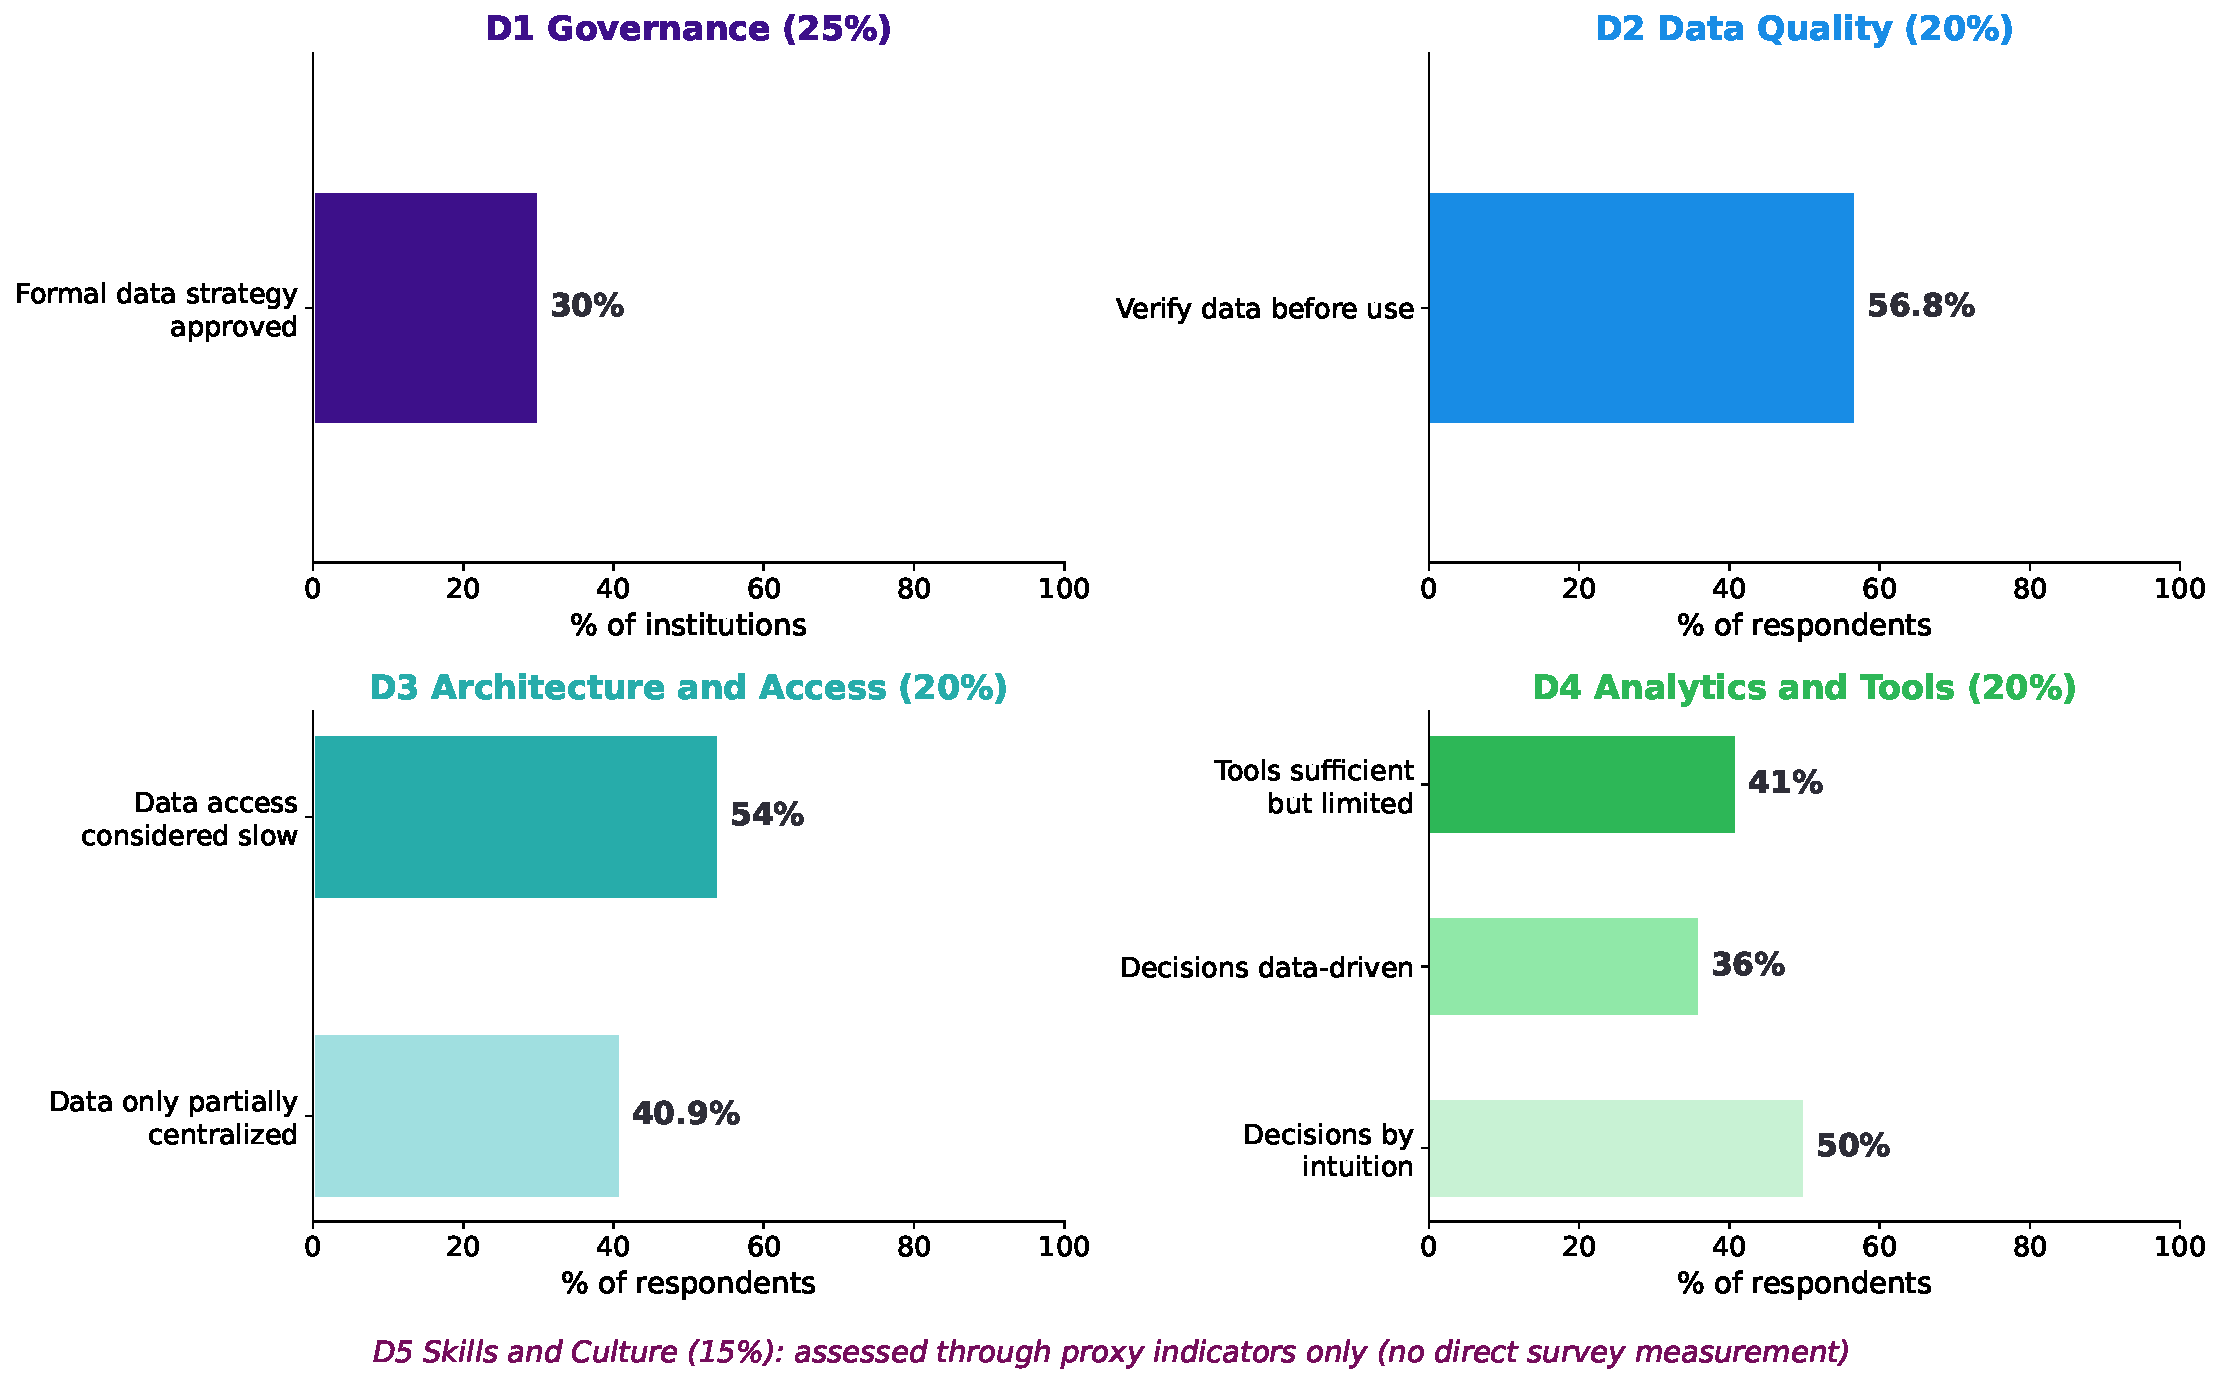
\includegraphics[width=\textwidth]{images/survey-findings.pdf}
\caption{Diagnostic survey findings across the five dimensions (44 respondents)}
\label{fig:survey}
\end{figure}

\subsection{Resulting Maturity Profile}

A representative maturity profile at Level 2 Emerging, consistent with the sector diagnostic, is illustrated in Figure~\ref{fig:radar-profile}. Its per-dimension scores and their contribution to the Global Maturity Index through the weighted aggregation formula are detailed in Table~\ref{tab:profile-breakdown}. The example yields a GMI of 2.19 out of 5, equivalent to 44\%, placing the institution at Level 2.

\begin{figure}[H]
\centering
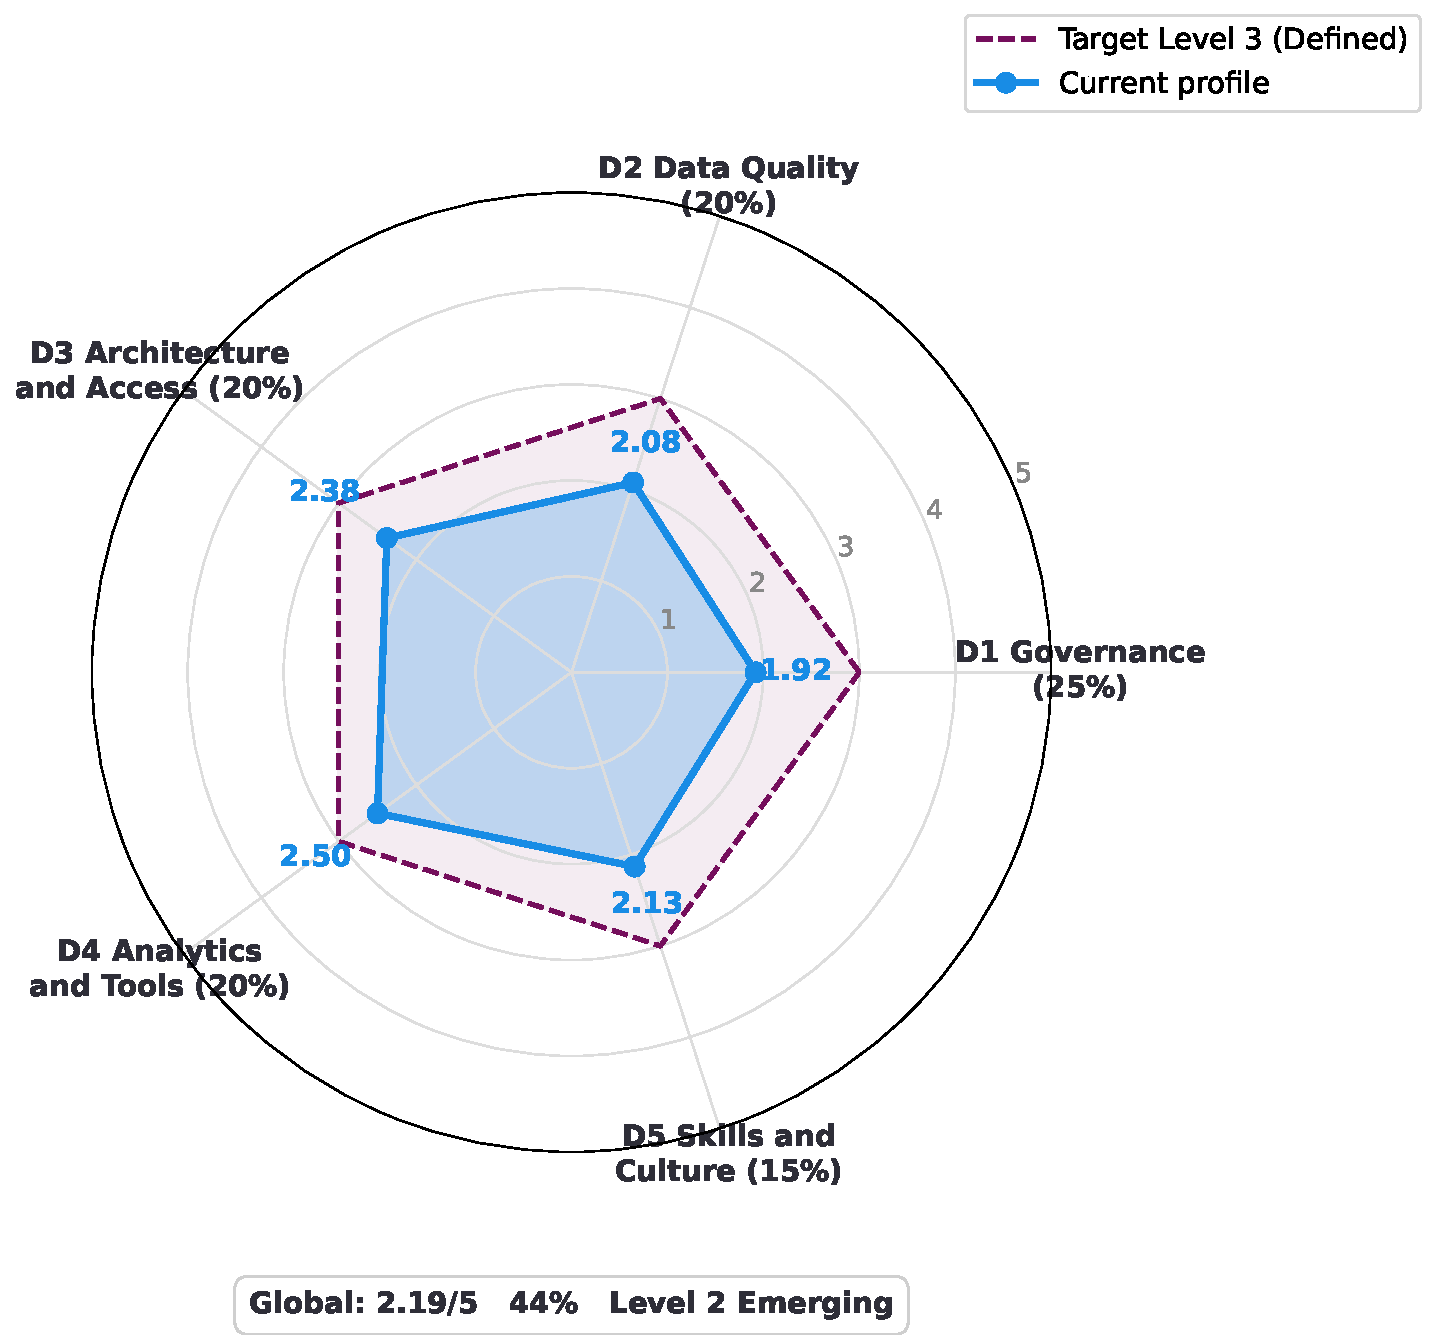
\includegraphics[width=0.75\textwidth]{images/radar-profile.pdf}
\caption{Sample maturity profile across the five dimensions (representative Level 2 bank)}
\label{fig:radar-profile}
\end{figure}

\begin{table}[H]
\centering
\caption{Composition of the Global Maturity Index for a representative Level 2 institution} \label{tab:profile-breakdown}
\begin{tabular}{|p{4.6cm}|c|c|c|}
\hline
\textbf{Dimension} & \textbf{Score (/5)}$^{\mathrm{a}}$ & \textbf{Weight} & \textbf{Weighted contribution} \\
\hline
D1 Governance & 1.92 & 25\% & 0.480 \\
D2 Data Quality & 2.08 & 20\% & 0.416 \\
D3 Architecture and Access & 2.38 & 20\% & 0.476 \\
D4 Analytics and Tools & 2.50 & 20\% & 0.500 \\
D5 Skills and Culture$^{\mathrm{b}}$ & 2.13 & 15\% & 0.320 \\
\hline
\textbf{Global Maturity Index}$^{\mathrm{c}}$ & & \textbf{100\%} & \textbf{2.19 / 5 (44\%)} \\
\hline
\end{tabular}
\par\vspace{4pt}
\parbox{12.5cm}{\footnotesize
$^{\mathrm{a}}$ Dimension scores are effective scores, that is, scores computed after the application of the evidence cap, so an unsupported high answer has already been reduced before entering this table.
$^{\mathrm{b}}$ Skills and Culture is assessed through proxy indicators only, and none of the thirteen regulatory indicators belongs to this dimension.
$^{\mathrm{c}}$ All five dimensions are answered in this example, so the renormalization leaves the nominal weights unchanged and they sum to 100\%. The dimension scores are the tool's two-decimal display values; the engine aggregates the unrounded dimension means at full precision, which yields the reported index of 2.19, so the rounded per-dimension contributions above reconcile to 2.19 up to display rounding. This example is fully reproducible from a stored answer set and is the same session captured in the DataPilot screenshots of Chapter~4.}

\end{table}

The composition in Table~\ref{tab:profile-breakdown} makes the aggregation explicit. Each dimension score is multiplied by its weight, and because all five dimensions are answered, the weights sum to 100\% and no renormalization is required. The weighted contributions, 0.480, 0.416, 0.476, 0.500, and 0.320, add to 2.19, which the percentage conversion turns into round(2.19 times 20) equal to 44\%. The value 2.19 falls inside the 1.80 to 2.59 band (defined in Appendix~E, with the level rubrics in Appendix~A), placing the institution at Level 2, Emerging. Were one dimension left unanswered, its weight would be removed from the denominator and the remainder rescaled to 100\%, so the index reflects only the dimensions actually assessed rather than silently scoring a missing dimension as zero. The reported level is, moreover, robust to the exact weighting. Shifting each of the nominal weights of 25/20/20/20/15 by up to five percentage points and renormalizing, the index of this profile varies only between about 2.14 and 2.24; under equal weights it is 2.20, every value well inside the Level 2 Emerging band. The weighting thus fixes the emphasis and ordering of the dimensions, while the reported level is not sensitive to the precise weights chosen.

The profile also illustrates a critical gap. Governance, at 1.92 out of 5, sits below the 2.0 threshold and is flagged as a critical gap: a dimension under 2.0 signals a weakness serious enough to require priority attention regardless of the overall index. This 2.0 gap threshold is deliberately distinct from the 1.80 lower bound of the Level 2 band; the band labels the overall maturity level, whereas the gap threshold flags a single dimension for priority action, so a dimension can sit inside the Emerging band and still be flagged, as governance is. It is the only dimension flagged, since every other score exceeds 2.0. Data quality, at 2.08, is the second weakest and, just above the threshold, is not flagged but is the natural next target once governance is addressed. Analytics, at 2.50, and architecture, at 2.38, are the relative strengths, though they too remain within the emerging band and well short of the defined level.

Taken together, the findings describe a sector concentrated at the emerging level. Governance and data quality are the weakest dimensions, held back by the absence of formal strategy and automated control, while architecture and analytics show partial progress. This profile is the baseline against which individual institutions can be positioned using the framework and DataPilot, and against which improvement can be steered.

\subsection{From Profile to Improvement Roadmap}

The maturity profile has value only when converted into action. DataPilot performs this through its gap analysis, which operates at the twelve sub-dimensions rather than the five dimensions, so guidance targets the specific weak practice rather than a whole dimension. Each sub-dimension is assigned a priority on a deterministic four-level scale mirroring the scoring thresholds: critical below 2.0, high below 2.6, moderate below 3.4, and low at 3.4 and above. These priorities are grouped into a three-phase, time-sequenced roadmap, but the grouping is not a simple copy of the label, because regulatory risk can override it: a sub-dimension containing a failing regulatory indicator, or scoring below 2.0, goes to the first phase regardless of its numeric priority. The remaining sub-dimensions short of the defined level go to the second phase, and those that have reached it go to the third. Each sub-dimension card surfaces a small, bounded set of concrete actions, so the roadmap is specific rather than open-ended.

Applied to the representative profile, this logic yields a clear sequencing, shown in the gap analysis screen of Chapter~4. Five sub-dimensions fall in the first phase: the two weakest governance sub-dimensions, strategy and data policy and ownership and responsibilities, both below 2.0; the governance regulatory-compliance sub-dimension, pulled in not by its score but because it still carries a failing regulatory indicator, audit readiness; and the data-quality controls and processes and data-skills proxy sub-dimensions, both below 2.0. Their first-phase actions include formally approving a data strategy document at board level, appointing a chief data officer or equivalent with an executive mandate, establishing a data governance committee with a formal charter, and closing the two open regulatory gaps in governance. The remaining seven sub-dimensions, all between 2.0 and 3.0 here, fall in the second phase, with actions such as automating key data quality controls in critical pipelines, integrating all major business lines into a centralized platform, documenting end-to-end lineage, and launching self-service analytics with user training. The third phase is empty, because no sub-dimension has yet reached the defined level; its optimization actions, such as predictive quality monitoring or measuring data culture adoption through an annual index, are staged for when a sub-dimension crosses into the defined level.

The three phases correspond to increasing maturity and a time horizon. The first, over the first three months, remediates the critical gaps and open regulatory items and establishes the missing foundations; the second, over three to six months, automates and integrates the partially mature sub-dimensions; the third, over six to twelve months, optimizes and benchmarks those that have reached the defined level. Figure~\ref{fig:roadmap} presents this model and the representative action themes for each phase.

\begin{figure}[H]
\centering
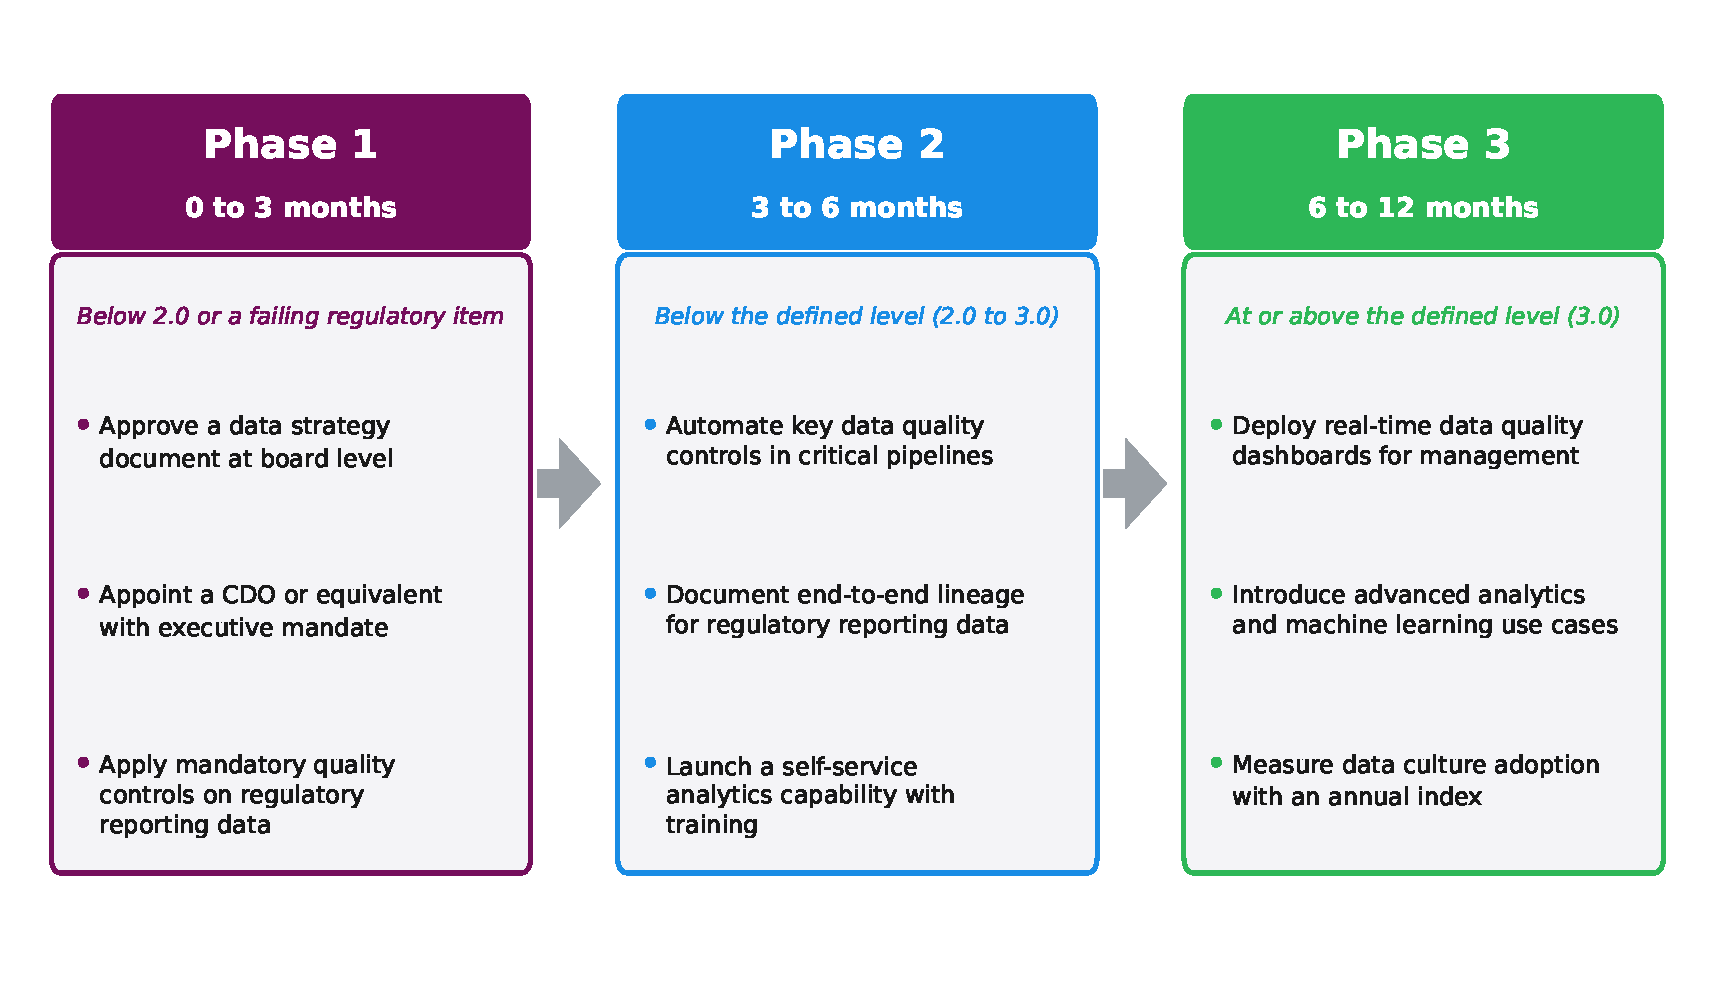
\includegraphics[width=0.85\textwidth]{images/roadmap.pdf}
\caption{Three-phase improvement roadmap derived from the gap analysis}
\label{fig:roadmap}
\end{figure}

The roadmap is not merely a presentation device. The banding derives directly from the same scores that produce the index, so the sequence of actions is auditable and reproducible: two assessors who enter the same raw scores obtain the same bands and the same ordered actions. This is computational reproducibility, not inter-rater agreement, since two assessors may read the same rubric and evidence yet enter different raw scores; that distinction is examined in the Discussion. This determinism makes the roadmap a steering instrument rather than a consultative opinion, and lets an institution re-run the assessment after an intervention and observe a dimension move out of the critical band toward the defined level.

\subsection{An Assessment Session End to End}

This walkthrough follows the solo assessment path delivered in the single-user build of Iteration 3, whose screens are the captures shown in Chapter 4. In the Iteration 4 platform, session identity comes from the analyst's invited account rather than a typed form, and a completed solo assessment can additionally be submitted for review to the bank's administrators; the multi-tenant flows, including the collaborative group assessment, are specified in Iteration 4. The results above are produced through one continuous workflow, and following a complete session from the assessor's seat shows how the instrument behaves where its rules matter, tracing the journey summarized in Figure~\ref{fig:user-journey}. A session opens on the Welcome screen, where the assessment cannot begin until the inline profile form, covering bank name, date, respondent name, and role, is complete and the start action becomes available. The questionnaire then presents the forty seven indicators grouped by dimension and sub-dimension, beginning with the twelve governance indicators. For each, the assessor reads the question and the five level rubric, selects a score, and documents the supporting evidence. The business rules act at the moment of entry, not at the end: an indicator scored four with its evidence field left empty is immediately computed and displayed as a two and flagged as capped; the skip control is disabled on the thirteen regulatory indicators, and a request to skip a third governance indicator is refused, the ceiling for that dimension being two. Only when the forty seventh indicator has been answered or lawfully skipped does the completion gate open the results, gap analysis, and compliance views, which until then redirect back to the questionnaire. Figures~\ref{fig:screen-questionnaire} through~\ref{fig:screen-compliance} in Chapter 4 show these screens as captured from a complete demonstration session.

The representative Level 2 institution of Table~\ref{tab:profile-breakdown} is the same session captured in the DataPilot screenshots of Chapter 4, so its figures can be read directly off those screens. The results dashboard displays the Global Maturity Index, its percentage form, and the Level 2 Emerging badge, and the radar chart overlays the five dimension scores of Table~\ref{tab:profile-breakdown} on the selected target level. The gap analysis reads the same stored scores, flags governance as the single critical gap, and places the two weakest governance sub-dimensions and the still-open governance regulatory items in the first phase alongside the other sub-dimensions below 2.0, while the rest fall into the second phase. Nothing on these screens is computed anew: every figure is a projection of the same stored answers through the aggregation chain of the design iterations, which is what allows any displayed number to be retraced by hand (Appendix~E).

The compliance view closes the session by classifying the regulatory core, and its mechanics can be made concrete on the same session, shown in the Results and Compliance screenshots of Chapter 4, Figures~\ref{fig:screen-results} and~\ref{fig:screen-compliance}. The rule is the one defined in the design iterations: each of the thirteen regulatory indicators is classified from its effective score, compliant at three out of five or above, non-compliant below that, and pending when unanswered. The threshold sits at three because level three is where an obligation is formalized, documented, and demonstrable rather than merely intended. The compliance rate is the compliant share of the thirteen, rounded to a percentage, and exposure is rated low from 80\% upward, medium from 50\% upward, and high below that, exactly as set out in Appendix~E. These exposure bands are an operational classification chosen to give management a simple risk signal, not a regulator definition; for a formal compliance exercise, any non-compliant regulatory indicator would require remediation regardless of the aggregate rate. In the captured session, ten of the thirteen regulatory indicators reach an effective score of three and are compliant; the remaining three, each at an effective score of two and all in governance, are non-compliant, and none is pending since the session is complete. The rate is therefore round(10/13 times 100) equal to 77\%, and because 77\% lies between the 50\% and 80\% thresholds, the regulatory exposure is rated medium. This session, whose profile is in Table~\ref{tab:profile-breakdown}, sits within the emerging band, and its summary shows what the compliance view adds to the index: an institution can be three indicators away from a low exposure rating and know exactly which three, since each non-compliant line names its indicator, dimension, regulatory reference, and supporting evidence.

\subsection{Answers to the Research Questions}

Drawing on the diagnostic findings, the maturity profile, and the artifacts above, this section answers each of the three research questions and its sub-questions in turn.

\subsubsection{RQ1 Answer}

\textbf{In short: the sector sits at the emerging level (Level 2), with governance and data quality the weakest and most exposed areas.} Data maturity in Tunisian banks is concentrated at the emerging level, with the main gaps relative to international standards and regulatory requirements in governance and data quality. Most institutions lack a formally approved data strategy and rely on manual rather than automated quality control, placing them below the governance and control expectations of the BCT Circulaire N\textdegree{}2025-08 and BCBS 239. The diagnostic and the framework together make these gaps measurable and explicit.

In answer to RQ1a, the diagnostic evidence locates these gaps dimension by dimension. Governance is weakest, because the strategy layer that should mandate ownership, stewardship, and regulatory alignment is reported in place by only a minority of respondents. Data quality is second weakest, because verification remains a manual behavior rather than an automated, monitored control, precisely where BCBS 239 and the reliability of regulatory reporting are most sensitive. Architecture and analytics are further along, with partial centralization and partly sufficient tooling, but neither reaches the defined level, both held back by incomplete automation and residual silos. Skills and culture cannot be measured directly and is inferred through proxy indicators. In answer to RQ1b, the survey evidence indicates that non-compliance concentrates on the governance obligations, particularly the formally approved data strategy and audit readiness. For a single institution, the instrument quantifies the compliance rate over the thirteen non-skippable indicators and the exposure it implies. The survey itself yields no sector-wide compliance rate: the 77\% rate and Medium exposure reported here are for the single demonstration session only, and establishing a sector-wide rate would require the field pilot assessments identified in future work. The overall picture is a sector aware of the importance of data and beginning to invest, but not yet having institutionalized the strategy, control, and automation that would move it from emerging to defined. The gaps are not diffuse impressions but specific, indicator-level deficiencies that the framework can locate and the tool can track.

\subsubsection{RQ2 Answer}

\textbf{In short: a hybrid framework was designed that fuses five established benchmarks into five dimensions, twelve sub-dimensions, and forty seven indicators, scored by an evidence-capped weighted Global Maturity Index.} A data maturity assessment framework adapted to the Tunisian banking sector was designed by combining established benchmarks with the survey findings. In answer to RQ2a, the comparative analysis showed that each of the five frameworks contributes a distinct strength, DAMA-DMBOK its structure, DCAM its regulatory alignment, CMMI its scale, TDWI its evaluation logic, and Gartner its executive communication, and that no single framework suffices alone. In answer to RQ2b, the framework was structured around five dimensions, twelve sub-dimensions, and forty seven indicators, with a five level maturity scale and a weighted scoring methodology that produces an auditable Global Maturity Index (GMI) on a one to five scale.

The adaptation to the local context distinguishes the framework from a direct import of any single benchmark. The five dimensions are weighted at 25\%, 20\%, 20\%, 20\%, and 15\%, giving governance the largest influence in recognition of its regulatory centrality in Tunisian banking. Thirteen of the forty seven indicators are flagged regulatory and non-skippable, mapped to specific requirements of the BCT Circulaire N\textdegree{}2025-08 and the BCBS 239 principles, so regulatory readiness is measured within the same instrument as maturity rather than separately. The methodology further embeds an evidence cap, preventing an unsupported high score from inflating the result, and a bounded skip mechanism that excludes skipped indicators from the denominators while forbidding any skip of a regulatory indicator. The result is a framework at once standard-aligned, locally adapted, and auditable, as the research question asked.

\subsubsection{RQ3 Answer}

\textbf{In short: DataPilot operationalizes the framework into auditable automated scoring, dashboards, a prioritized improvement roadmap, and a regulatory compliance view.} The interactive tool supports strategic decision-making by turning a static assessment into an actionable instrument: it automates scoring, presents the maturity profile through dashboards, prioritizes improvement actions through a gap analysis, and reports regulatory readiness through a compliance view. By making the maturity state and improvement path explicit and auditable, the tool gives bank management a concrete basis on which to steer their data strategy and accelerate their digital transformation.

Concretely, the tool closes the distance between assessment and action along four axes. In answer to RQ3a, it removes manual computation error by applying the aggregation chain, evidence cap, renormalization, and percentage conversion consistently, so the reported index is always reproducible, resistant to over-optimistic self-assessment, and, when the same dimensions are assessed, comparable across institutions. It makes the profile legible to non-specialists through a radar chart, dimension bars, and a maturity badge naming the level. In answer to RQ3b, it converts the profile into a sequenced roadmap by banding each dimension score and surfacing the corresponding actions, giving management an ordered set of interventions rather than a raw diagnosis. And it exposes regulatory exposure directly, evaluating the thirteen regulatory indicators, reporting a compliance rate, and classifying residual exposure as low, medium, or high. Because all of this derives from a single stored answer set recomputed on demand, the tool also supports the re-assessment cycle that turns a one-time diagnosis into ongoing steering. Demonstrating that a real institution's transformation was in fact accelerated would require the field pilot identified in future work, and no such claim is drawn from the functional evaluation here. The platform delivered in Iteration 4 extends this support to the scale of the institution: departments contribute their assigned dimensions within a group assessment, a coordinator consolidates the work into one auditable submission per bank, and EY reviews submissions across banks. The same instrument thus steers the transformation of a whole organization rather than a single assessor's session.

\subsection{Conclusion}

This chapter reported the sector diagnostic findings dimension by dimension, summarized the resulting maturity profile and its composition into the Global Maturity Index, explained how that profile is translated into a three-phase improvement roadmap, and answered the three research questions. The next chapter discusses these results, their implications, and the threats to validity.
